\documentclass[12pt]{article}
\usepackage[utf8]{graphicx}
\graphicspath{{./Images/}}

\title{The Monkey and the Hunter Problem}
\author{Lauren Bourque }
\date{November 12, 2018}

\begin{document}

\maketitle

\section{The Problem}
A clever monkey is in a tree six meters above the ground. A hunter, 8 meters from the tree, shoots a tranquilizer dart at the monkey. The monkey lets go of the tree at the same instant that the dart leaves the gun, intending to land on the ground and escape. Under what conditions, if any, will the dart hit the monkey? Where should the hunter aim and how does the initial speed of the dart affect the shot?
\section{Drawing a Picture}
To best understand all of the given information, a picture can be drawn that displays the problem.\\
\begin{center}
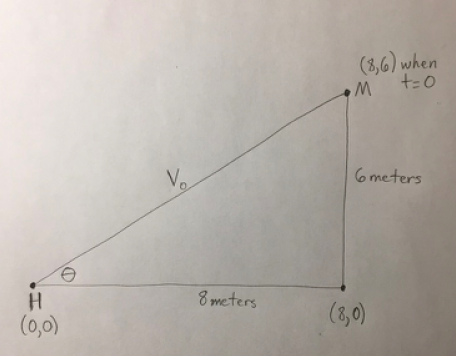
\includegraphics[scale=0.5]{picture}
\end{center}
\section{Interpretations of the Picture}
There is a lot of information, but it can be explained.\\\\
In this picture, the hunter is considered variable $H$. He is set at point $(0,0)$ on the x and y axes to make the problem easier to understand. \\\\
$H$ is 8 meters away from the base of the tree whose coordinates are $(8,0)$ on the x and y axes.\\\\
Directly 6 meters above this point, the monkey is positioned in the tree. It is considered variable $M$ and sits at point $(8,6)$ on the x and y axes. Since this is the monkey's initial position, it was sitting there at time t=0.\\\\
Since the velocity of the dart is unknown, it can be listed as a variable to be found, $v_0$.\\\\
Since the angle that the dart is shot at is also unknown, it can be listed as a variable to be found, $\theta$.\\\\
Since two sides of the triangle are listed, trigonometry can be used to find the angle $\theta$.
$$tan(\theta)=\frac{6}{8}$$
Isolate $\theta$.
$$\theta=arctan(\frac{3}{4})$$
This new value of $\theta$ will eventually be helpful in solving the problem.
\section{Writing Parametric Equations}
Prior knowledge can be used to create parametric equations (displaying x and y over time, t) to manipulate the problem. Let $D(x,y)$ be listed as the equations for the dart as it travels over time. Let $M(x,y)$ be listed as the equations for the monkey as it travels over time.\\
$$x_D=v_{0}t\cdot cos\theta$$
This represents the equation for the x values of the dart over time. $v_0$ was multiplied by t because it represents how the unknown velocity of the dart traveled over time, $t$. This is why $v_0$ was multiplied by $t$. This was also multiplied by $cos\theta$ because $cos\theta$ represents the angle of the dart over the x-axis. This equation represents how far the dart traveled and when.
$$y_D=v_{0}t\cdot sin\theta-4.9t^2$$
This represents the equation for the y values of the dart over time. $v_0$ was multiplied by t because it represents how the unknown velocity of the dart traveled over time, $t$. This is why $v_0$ was multiplied by $t$. This was also multiplied by $sin\theta$ because $sin\theta$ represents the angle of the dart over the y-axis. $4.9t^2$ was subtracted from the equation because it represents the value of the acceleration of gravity in meters per second over time. This equation represents how high the dart traveled and when.
$$x_M=8$$
This represents the equation for the x values of the monkey over time. Since the monkey drops straight down in line with the tree from the tree's top and the tree is 8 meters away from the hunter, the monkey will always be 8 meters away from the hunter. This is why $x_M$ always equals 8.
$$y_M=6-4.9t^2$$
This represents the equation for the y values, or the height of the monkey over time. Since the monkey begins at a height of 6 meters, the value of 6 is written in the equation as the maximum height. $4.9t^2$ was subtracted from the equation because it represents the value of the acceleration of gravity in meters per second over time.
\section{Using the Parametric Equations}
Since the first question to answer is when the dart will hit the monkey, the x equations for the two parametrics must be set equal to each other to find the time that the monkey and the dart collide at the same length. The y equations for the two parametrics must also be set equal to each other to find the time that the monkey and the dart collide at the same height. Since a t value is what is being found but t is already used in the equations, $t_n$ will be the variable to find.
$$x_D(t_n)=8$$
$$x_M(t_n)=v_{0}t_n\cdot cos\theta$$
$$x_D(t_n)=x_M(t_n)$$
$$v_{0}t_n\cdot cost=8$$
Isolate $t_n$.
$$v_0t_n=\frac{8}{cos\theta}$$
$$t_n=\frac{8}{v_{0}cos\theta}$$
This variable will be used to solve the two y parametric equations and to determine when the y values or heights are equal to each other.
$$y_{D}(t_n)=y_M(t_n)$$
First, try solving $y_D(t_n)$ to see if information from the simplified equation can be used to set equal to $y_M(t_n)$ to find the time that they're equal.
$$y_D(t_n)=v_{0}(t_n)\cdot sin\theta-4.9(t_n)^2$$
This can be rewritten.
$$y_D(t_n)=v_{0}(\frac{8}{v_{0}cos\theta})\cdot sin\theta-4.9(\frac{8}{v_{0}cos\theta})^2$$
This can be simplified.
$$y_D(t_n)=8tan\theta-4.9(\frac{8}{v_{0}cos\theta})^2$$
This can be rewritten by substituting in $tan\theta$.
$$y_D(t_n)=8(\frac{6}{8})-4.9(t_n)^2$$
This can be further simplified.
$$y_D(t_n)=6-4.9(t_n)^2$$
Now, try to find $y_M(t_n)$.
$$y_M(t_n)=6-4.9(t_n)^2$$
Eureka! It can be seen that $y_D(t_n)=y_M(t_n)$. This means that at any point, the dart and the monkey will have an equal height. This means that the dart will always hit the monkey, no matter the monkey's height, as long as the velocity reaches the minimum value necessary to get the dart to the tree. Therefore, as long as the dart has this minimum velocity, the hunter should aim at the monkey because he will always hit it.\\\\
However, the minimum velocity required should be found to make sure that the hunter's dart is moving fast enough to hit the monkey.
\section{Finding the Minimum Velocity}
How does a different value for velocity alter the problem?\\\\
To find the minimum velocity required for the dart to hit the monkey, this question must be explored.\\
To be able to see this best, the differential equations were graphed in the x and y axes over t with the velocity set at 100 meters per second.\\\\
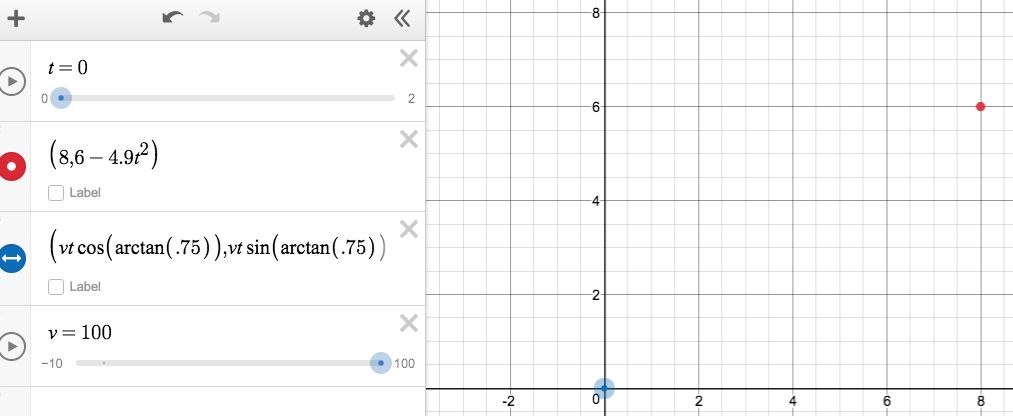
\includegraphics[scale=0.48]{picture1}
\begin{center}
    This is the velocity at 100 meters per second at t=0.
\end{center}
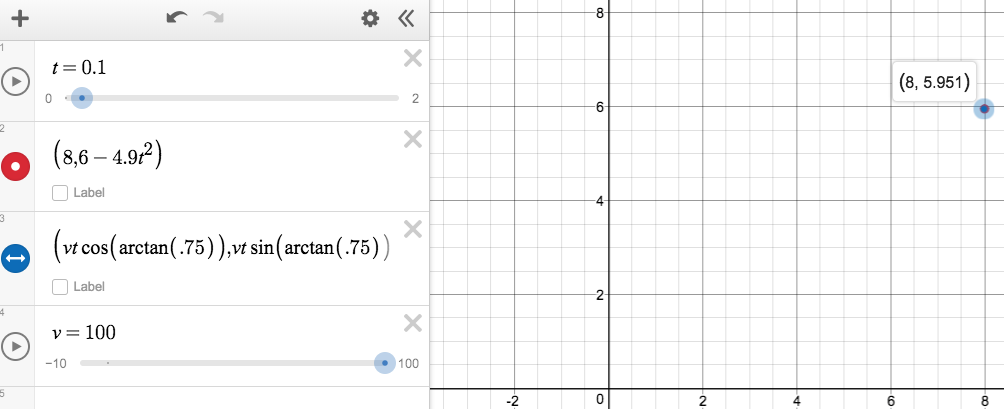
\includegraphics[scale=0.48]{picture2}
\begin{center}
    This is the velocity at 100 meters per second at t$\approx$0.1.
\end{center}
From this image, it can be seen that when t is about 0.1 and the velocity is at 100 meters per second, the dart reaches the monkey at a height of 5.951. This is when the dart hit the monkey because it reached an x value of 8, being enough to hit the tree. The tall height shows that the monkey didn't fall very far before it was hit by the dart.\\\\
To see the difference in time that the dart hits the monkey, the differential equations were graphed again with the velocity set at 10 meters per second.\\\\
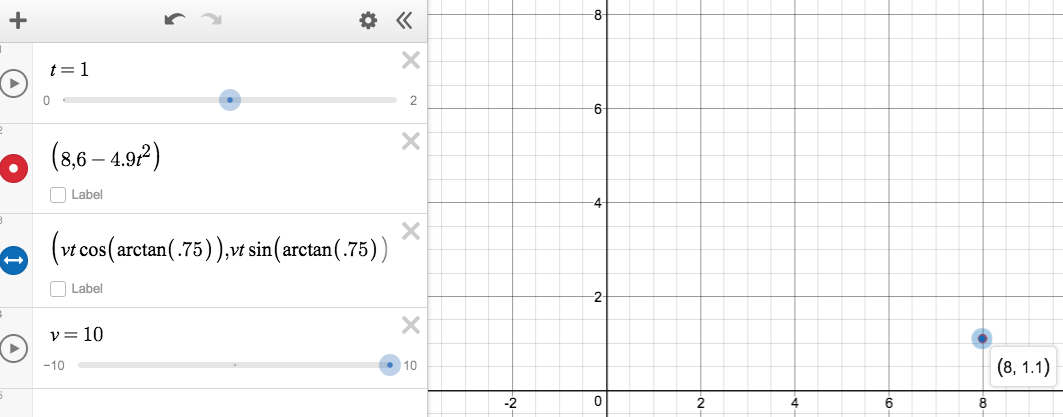
\includegraphics[scale=0.45]{picture3}
\begin{center}
    This is the velocity at 10 meters per second at t$\approx$1.
\end{center}
From this, it can be seen that when t is about 1 and the velocity is at 10 meters per second, the dart reaches the monkey at a height of 1.1. This height is much shorter and much closer to the ground. From this, it can be concluded that the minimum velocity possible for the equation would exist when the dart hits the monkey at a height of 0.\\\\
To first find the time value, 0 will be set equal to the monkey's height, or $y_M$.
$$0=6-4.9t^2$$
$$-6=-4.9t^2$$
$$\frac{6}{4.9}=t^2$$
$$\sqrt{\frac{6}{4.9}}=t\approx1.1065666703$$
This value should be substituted into the equation of the length reached by the dart, or $x_D$. 8 will be substituted in for the value of $x_D$ because it's the length that has to be reached for the dart to hit the monkey.
$$8=v_{0}\sqrt{\frac{6}{4.9}}\cdot cos(arctan(\frac{3}{4}))$$
$$v_{0}=\fbox{9.03696114115 meters per second}$$
This is the minimum velocity required for the dart to hit the monkey, which can be proven by the graph below.\\\\
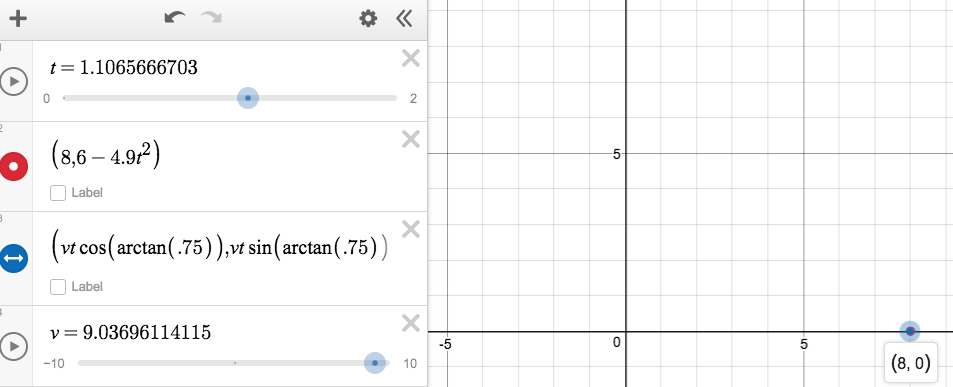
\includegraphics[scale=0.48]{picture4}
\begin{center}
    This is the velocity at 9.03696114115 meters per second at t$\approx$1.1065666703.
\end{center}
\end{document}
